\section{Method: TissuePMHC Model for Human Data}

\subsection{Model Overview and Tissue--HLA-specific Prediction}

Peptide presentation contains sequence patterns at more than one biological level. Some features may recur across many tissues and HLA alleles, whereas others may reflect motifs associated with one allele. TissuePMHC therefore contains a global pathway that learns from all tissue--HLA combinations with additional tissue and allele supervision, and an HLA-specific pathway that learns only from combinations sharing one HLA allele. Each pathway produces a separate score for every tissue--HLA combination. Their within-combination rankings are combined with equal weight and then averaged across three independently trained models.

Both pathways use a position-aware peptide encoder that preserves residue position and examines neighboring residues, followed by a separate output layer for each observed tissue--HLA combination. This structure allows combinations with many examples to support those with fewer examples without forcing all alleles to use an identical peptide representation. Because the final prediction depends on an output layer learned for a particular combination, the model is not designed for tissue--HLA combinations absent from training.

\begin{figure*}[t]
\centering
\resizebox{0.82\linewidth}{!}{%
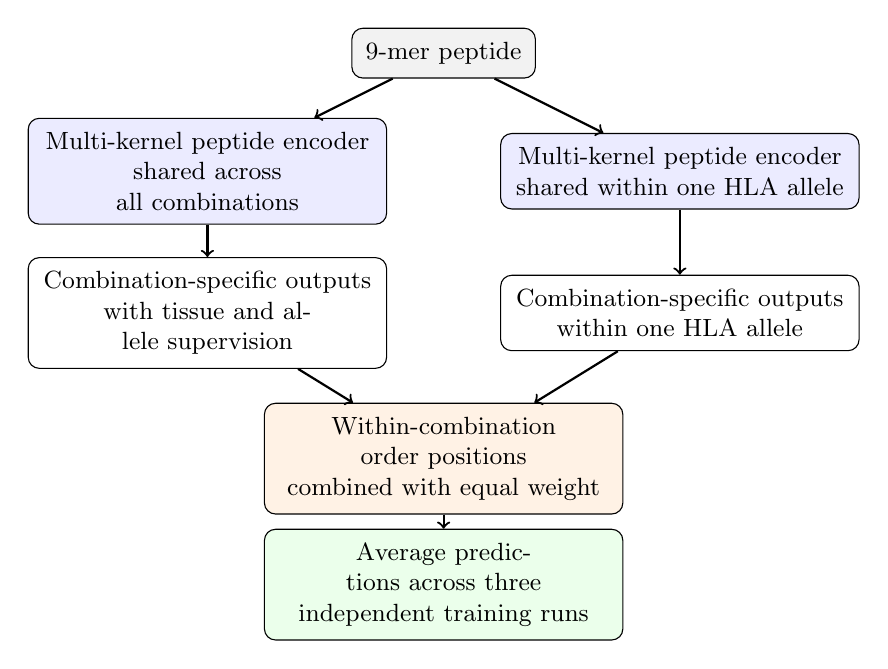
\begin{tikzpicture}[
    box/.style={draw,rounded corners,align=center,inner sep=5pt,font=\small},
    widebox/.style={box,text width=4.2cm},
    arr/.style={->,thick}
]
\node[box,fill=gray!10] (pep) at (0,0) {9-mer peptide};
\node[widebox,fill=blue!8] (encg) at (-3,-1.5) {Multi-kernel peptide encoder\\shared across all combinations};
\node[widebox,fill=blue!8] (ench) at (3,-1.5) {Multi-kernel peptide encoder\\shared within one HLA allele};
\node[widebox] (global) at (-3,-3.3) {Combination-specific outputs\\with tissue and allele supervision};
\node[widebox] (hla) at (3,-3.3) {Combination-specific outputs\\within one HLA allele};
\node[widebox,fill=orange!10] (fusion) at (0,-5.15) {Within-combination order positions\\combined with equal weight};
\node[widebox,fill=green!8] (ensemble) at (0,-6.75) {Average predictions across three\\independent training runs};
\draw[arr] (pep) -- (encg);
\draw[arr] (pep) -- (ench);
\draw[arr] (encg) -- (global);
\draw[arr] (ench) -- (hla);
\draw[arr] (global) -- (fusion);
\draw[arr] (hla) -- (fusion);
\draw[arr] (fusion) -- (ensemble);
\end{tikzpicture}
}
\caption{Overview of the human model. The global pathway learns peptide patterns across all tissue--HLA combinations, whereas the HLA-specific pathway shares information only among tissues with the same allele. Tissue and allele prediction provide training supervision but do not enter the final score. The two within-combination rankings are combined and averaged across three independent training runs.}
\label{fig:tissuepmhc-architecture}
\end{figure*}

The remainder of this section gives the exact implementation needed for reproduction. Let \(h_i\) denote the numerical representation of peptide \(p_i\), and let \(\tau_i\) denote its tissue--HLA combination. Each pathway maintains a separate linear output for every available combination. The corresponding logit is
\[
z_i=g_{\tau_i}(h_i),
\]
and the associated presentation-preference probability is
\[
q_i=\sigma(z_i),
\]
where \(\sigma\) is the logistic sigmoid. During each mini-batch update, examples are routed to the output layer for their tissue--HLA combination, while encoder parameters are shared according to the pathway definition. The main objective is binary cross-entropy with logits, denoted BCE:
\[
\mathcal{L}_{\mathrm{BCE}}
=
-\frac{1}{B}
\sum_{i=1}^{B}
\left[
y_i\log q_i+(1-y_i)\log(1-q_i)
\right].
\]
Although every benchmark pair contains one recorded-positive row and one pseudo-negative row, the model processes rows independently. Pair identifiers are not used during the forward pass or loss calculation.

\subsection{Peptide Encoding That Preserves Position and Examines Several Motif Lengths}

The biological meaning of an amino acid depends on its position in a 9-mer peptide: anchor residues involved in MHC binding are not interchangeable with residues at other positions. The encoder therefore preserves all nine positions while examining local patterns of several lengths. For a peptide \(p=(a_1,\ldots,a_9)\), each residue is mapped to a learned 16-dimensional embedding and combined with a learned positional embedding:
\[
X=E(p)+P \in \mathbb{R}^{9\times d},
\]
where \(E(p)\) contains the residue embeddings and \(P\) is a trainable \(9\times d\) positional representation shared across peptides. These positional embeddings distinguish the same amino acid at different locations, which is important because anchor and supporting positions in MHC-I ligands are not interchangeable.

The model operates only on canonical 9-mer peptides. No tissue transcriptomics, proteomics, parent-protein sequence, flanking sequence, or external binding score is supplied as input. Tissue and HLA information enter through the combination identifiers, combination-specific output layers, parameter-sharing structure, and auxiliary training labels rather than through additional omics measurements.

To examine local sequence patterns spanning two, three, or five residues, we apply one-dimensional convolutions with widths
\[
\mathcal{K}=\{2,3,5\}.
\]
For each \(k\in\mathcal{K}\), the input is transposed to a channels-first representation and processed as
\[
H_k
=
\operatorname{ReLU}
\left(
\operatorname{Conv1D}_{k}(X)
\right).
\]
Each convolution produces 32 feature maps. Padding retains local context at the peptide ends. For even kernel widths, symmetric padding produces one additional position; the final position is therefore cropped to retain a length of nine. Each pathway consequently yields
\[
H_k\in\mathbb{R}^{9\times 32}.
\]

The three sets of local patterns are joined while preserving their sequence positions. We deliberately avoid reducing the peptide to a position-free maximum or average, because the same short motif can have a different meaning at a different position:
\[
v
=
\operatorname{Flatten}
\left[
H_2;H_3;H_5
\right]
\in\mathbb{R}^{9\cdot32\cdot3}.
\]
The resulting vector is passed through a two-layer multilayer perceptron,
\[
h
=
\operatorname{MLP}(v)
\in\mathbb{R}^{128},
\]
Each hidden layer has 128 units with rectified linear unit activation. During training, dropout with probability 0.2 is applied after the first hidden layer. Flattening the position-specific feature maps allows identical local patterns at different peptide positions to contribute differently to the representation. The multi-kernel encoder is tailored to peptides of this single length; convolution itself is not presented as a methodological novelty.

\subsection{Information Sharing Across All Combinations and Within HLA Alleles}

The global pathway allows every tissue--HLA combination to contribute to a shared peptide representation. During training, auxiliary tissue and HLA classification objectives encourage this representation to retain biologically relevant grouping information. These objectives do not provide gene expression, protein abundance, or other molecular measurements. If \(c_i^{(t)}\) and \(c_i^{(m)}\) denote the tissue and HLA categories, respectively, the global objective combines BCE with categorical cross-entropy, denoted CE:
\[
\mathcal{L}_{\mathrm{global}}
=
\mathcal{L}_{\mathrm{BCE}}
+
\lambda_t
\mathcal{L}_{\mathrm{CE}}
\left(
\widehat{c}^{(t)},c^{(t)}
\right)
+
\lambda_m
\mathcal{L}_{\mathrm{CE}}
\left(
\widehat{c}^{(m)},c^{(m)}
\right),
\]
with prespecified weights
\[
\lambda_t=\lambda_m=0.1.
\]
The tissue and HLA predictions guide representation learning but do not enter the final peptide score. They provide auxiliary supervision rather than independent biological evidence.

The HLA-specific pathway shares information only among tissues with the same allele, preserving allele-associated peptide preferences that broad pooling could blur. For each HLA allele \(m\), we define
\[
\mathcal{T}_m
=
\{(t,m)\in\mathcal{T}\}.
\]
A separate encoder is trained on rows belonging to \(\mathcal{T}_m\), and each tissue--HLA combination in the group receives its own linear output layer. The objective for allele \(m\) is
\[
\mathcal{L}_{m}
=
\frac{1}{|\mathcal{D}_m|}
\sum_{i\in\mathcal{D}_m}
\mathcal{L}_{\mathrm{BCE}}
\left(
g^{(m)}_{\tau_i}(h_i^{(m)}),y_i
\right).
\]
This pathway has no auxiliary tissue or HLA classification objective. Because every example handled by one allele-restricted model shares the same allele, the pathway concentrates on allele-specific peptide patterns and variation among tissues under that restriction. It complements the global pathway: broad sharing can stabilize combinations with few examples, whereas allele-restricted sharing can preserve motif structure that unrestricted pooling may blur.

\subsection{Combining the Two Within-combination Orderings}

The two pathways are trained separately, so a score of 0.8 need not have the same calibration in both. We therefore combine their rankings rather than their raw scores. Within each tissue--HLA combination, every candidate is converted to a percentile rank. For combination \(\tau\), let \(q_{g,i}\) and \(q_{h,i}\) be the two scores for row \(i\):
\[
\begin{aligned}
r_{g,i}
&=
\operatorname{PercentileRank}_{\tau}(q_{g,i}),\\
r_{h,i}
&=
\operatorname{PercentileRank}_{\tau}(q_{h,i}).
\end{aligned}
\]
The equal-weight rank-fused prediction for one training run is
\[
s_i^{(b)}
=
\frac{r_{g,i}+r_{h,i}}{2}.
\]
Both pathways receive equal weight; no tissue or test set is used to choose a preferred pathway. This procedure answers a ranking question, not an absolute probability question. A peptide's percentile depends on the other candidates scored in the same batch, so adding or removing candidates can change its final rank. Prospective use would therefore require either a predefined candidate set or a prespecified reference distribution.

\subsection{Averaging Independent Training Runs and Its Scope}

Neural-network training can vary across random initializations. We therefore repeat the complete training procedure three times and average the resulting rankings \cite{lakshminarayanan2017deep}:
\[
s_{i,\mathrm{final}}
=
\frac{1}{B}
\sum_{b=1}^{B}
s_i^{(b)},
\qquad B=3.
\]
For each training run, the probabilities from both pathways are first converted to within-combination ranks and combined. The resulting scores are then averaged across runs. This aggregation order is used consistently for the saved internal test set, pair-preserving cross-validation, and cross-validation in which each held-out peptide is excluded from every training combination.

The averaged prediction is a single point estimate and should not be confused with training stability. We therefore report results from the individual runs as well as their prediction average, separating variation across initializations from the benefit of averaging.

\subsection{Species-specific Mouse Models}

The mouse analysis tests whether the same prediction problem is learnable in a second species; no human parameters are transferred to mouse. Mouse implementations are trained independently on the 24 tissue--H2 combinations and include simple sequence baselines, a shared encoder, and matched dual-branch models with and without auxiliary tissue and H2 supervision. These models follow the control definitions in the Experimental Setup and are compared on identical folds. Neural predictions in the peptide-separated analysis are averaged across five independent runs.
